% !TEX TS-program = xeLaTeX
\documentclass[aspectratio=169]{beamer}

% Package imports
\usepackage{fontspec}
\usepackage{epigraph}
\usepackage{xcolor}
\usepackage[percent]{overpic}

% custom options to make epigraph look good on a beamer slide
\renewcommand{\epigraphrule}{0pt}
\setlength{\epigraphwidth}{.9\textwidth}
\renewcommand{\textflush}{flushepinormal}

\newcommand\blfootnote[1]{%
  \begingroup
  \renewcommand\thefootnote{}\footnote{#1}%
  \addtocounter{footnote}{-1}%
  \endgroup
}

% default document font specifications
\setmainfont{FiraSans-Book}
\setsansfont{FiraSans-Book}
\definecolor{textcolour}{rgb}{255,255,255}

% Definign the Mozilla colour palette for presentations 
\definecolor{moz_dark_green}{RGB}{77,78,83}
\definecolor{moz_light_green}{RGB}{208,211,212}
\definecolor{moz_light_blue}{RGB}{0,150,221}
\definecolor{moz_dark_blue}{RGB}{0,33,71}
\definecolor{moz_accent_green}{RGB}{111,190,74}
\definecolor{moz_accent_yellow}{RGB}{255,203,0}
\definecolor{moz_accent_orange}{RGB}{255,149,0}
\definecolor{moz_accent_orange2}{RGB}{230,96,0}
\definecolor{moz_accent_red}{RGB}{193,56,50}


% Background for all slides set here
\setbeamertemplate{background canvas}{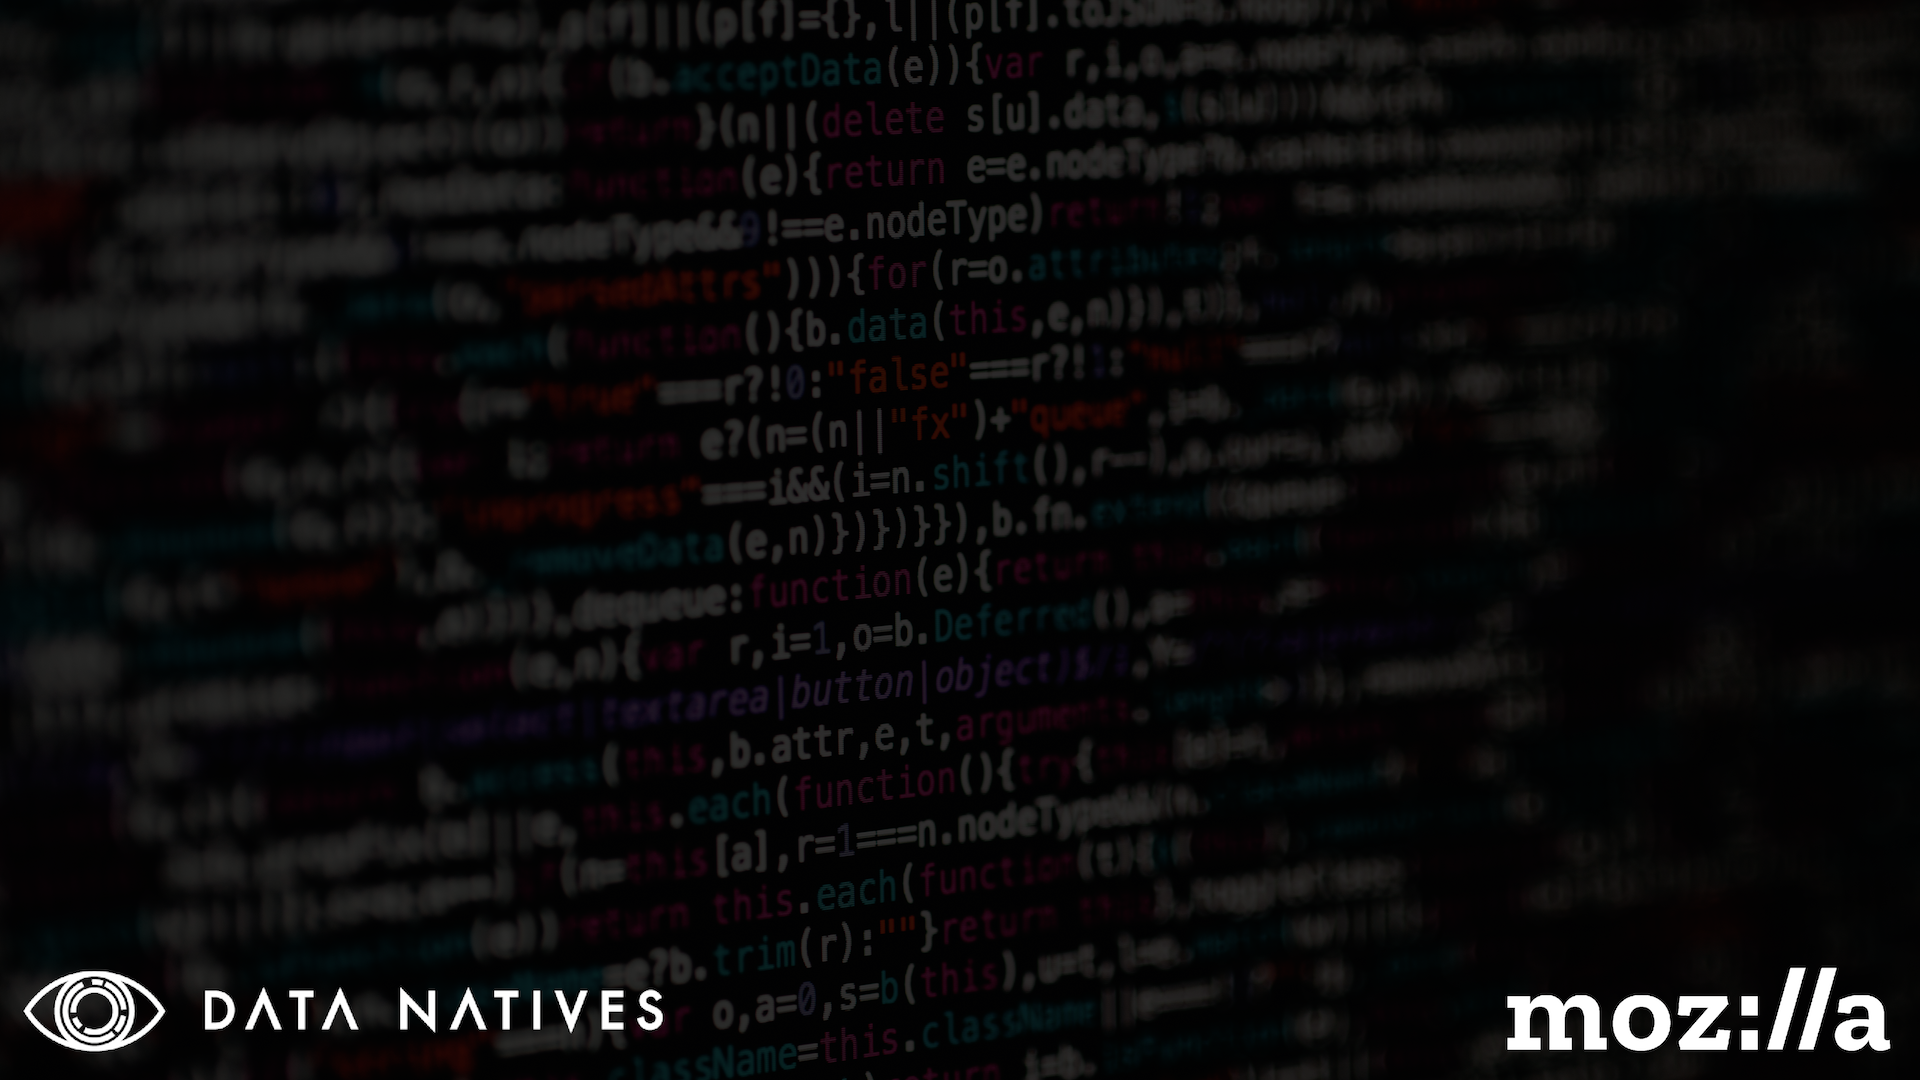
\includegraphics [width=\paperwidth]{bg_alt_small.png}}

\setbeamercolor{structure}{fg=textcolour}
\setbeamertemplate{items}[circle]

\setbeamerfont{title}{size = \Huge}
\setbeamercolor{normal text}{fg=textcolour}

%define specific fint size interpretations for the beamer presentation mode.
\renewcommand{\tiny}{\fontsize{7pt}{8pt}\selectfont}
\renewcommand{\scriptsize}{\fontsize{9pt}{12pt}\selectfont}
\renewcommand{\footnotesize}{\fontsize{10pt}{12pt}\selectfont}
\renewcommand{\small}{\fontsize{12pt}{18pt}\selectfont}
\renewcommand{\normalsize}{\fontsize{14pt}{18pt}\selectfont}
\renewcommand{\large}{\fontsize{16pt}{24pt}\selectfont}
\renewcommand{\Large}{\fontsize{24pt}{37pt}\selectfont}
\renewcommand{\LARGE}{\fontsize{36pt}{48pt}\selectfont}
\renewcommand{\huge}{\fontsize{48pt}{54pt}\selectfont}
\renewcommand{\Huge}{\fontsize{80pt}{96pt}\selectfont}

% remove navigation symbols
\setbeamertemplate{navigation symbols}{}
    
\begin{document}


\begin{frame}
\frametitle{The Morphology of the Web is Changing!}

% hey Data natives! it is absolutely great to be back for another iteration of this conference. 
%My name is Martin Lopatka, I work on Research Engineering and Data Science at Mozilla! 
%I'm here to talk to you about the Biggest data I know of...  The world’s largest shared public resource... The Web.
% So, we at Mozilla, work a bit on the web, we build a web browser, you may have heard of it.. it's called Firefox. 
% And, so as part of that, I'd say a pretty important part of that is knowing a thing or two about the World Wide Web.
% the story i want to talk about today has to do with its shape and a little bit about the technologies that define that shape
% One definition of Morphology is "the study of form and structure without consideration of function"

\begin{overpic}[width=0.7\textwidth]{morphs.png}
\put(45, 0){Form and structure of the modern Web} 
\end{overpic}

% So what got me started down this road: well a couple fo years ago, maybe around...  July 6th, 2016... at 11:16am.. Our VP of product Nick Nguyen made a medium post about the state of the web, 
\end{frame}

\begin{frame}
\frametitle{Disclaimer}
Martin Lopatka provides this contribution to the Data Natives 2018 conference in a personal capacity. The views expressed are his own and do not necessarily represent the views of Mozilla Corporation or the Mozilla Foundation.

% In addition on a personal note, this talk is not meant to be a vilification of the advertisement industry, or big companies, social media platforms, content publishers, or any other party. But rather, I want to focus on the changing nature fo the Web and what it means for technology and for people.
\end{frame}

{
\usebackgroundtemplate{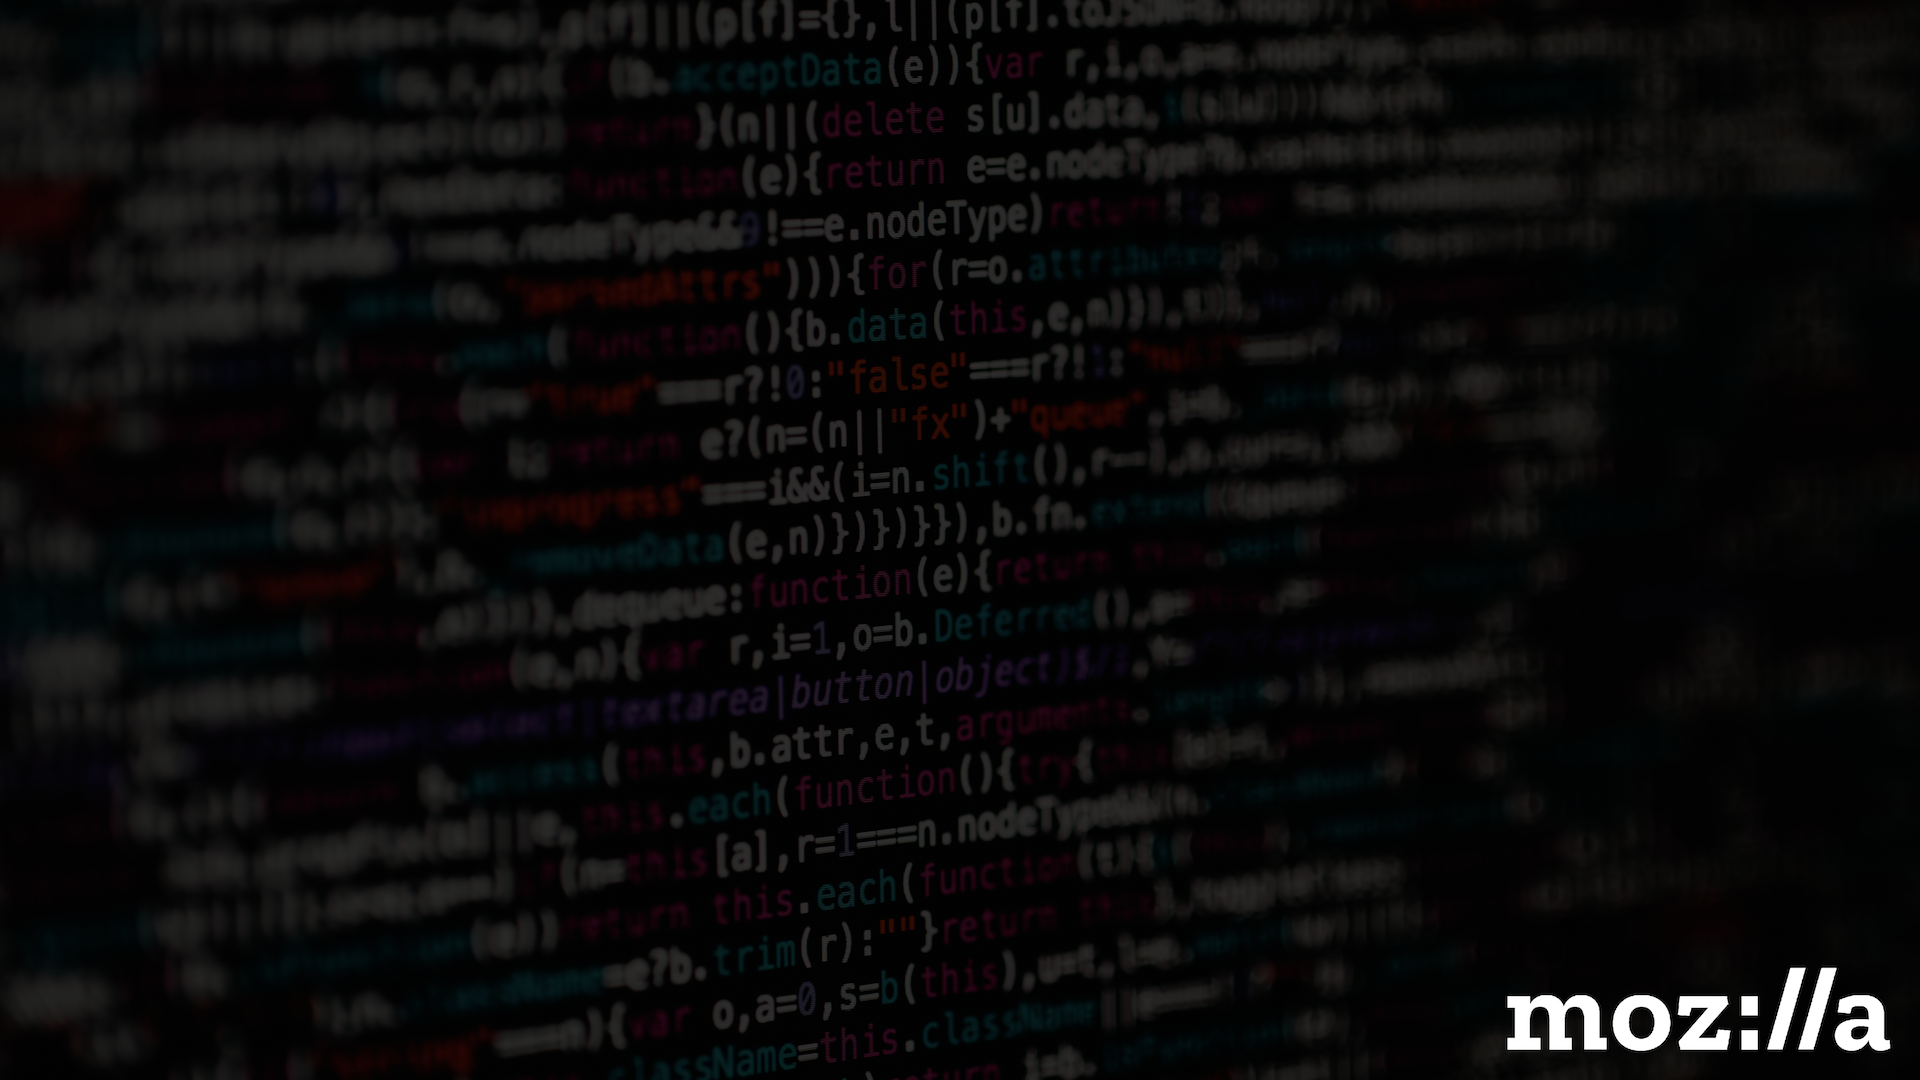
\includegraphics[width=\paperwidth]{bg_alt_small-rlogo.png}}%
\begin{frame}
\begin{overpic}[width=0.7\textwidth]{2003-web-small.png}
\put(-05,90){\textbf{THE INTERNET 2003}}
\put(-05,86){\tiny{Barrett Lyon / The Opte Project}}
%\blfootnote{Barrett Lyon / The Opte Project}
\end{overpic}
%This is our first full Internet map with color and other graphing logic. RFC1918 addresses have been hashed into a unique checksum so they do not incorrectly overlap with other routers or hosts. The checksums resolve to the same host each time to be sure that all routes connect correctly. Another bit of code also removed the routing loops that made a rather large mess out of previous maps. The colors were based on Class A allocation of IP space to different registrars in the world.
\end{frame}
}

{
\usebackgroundtemplate{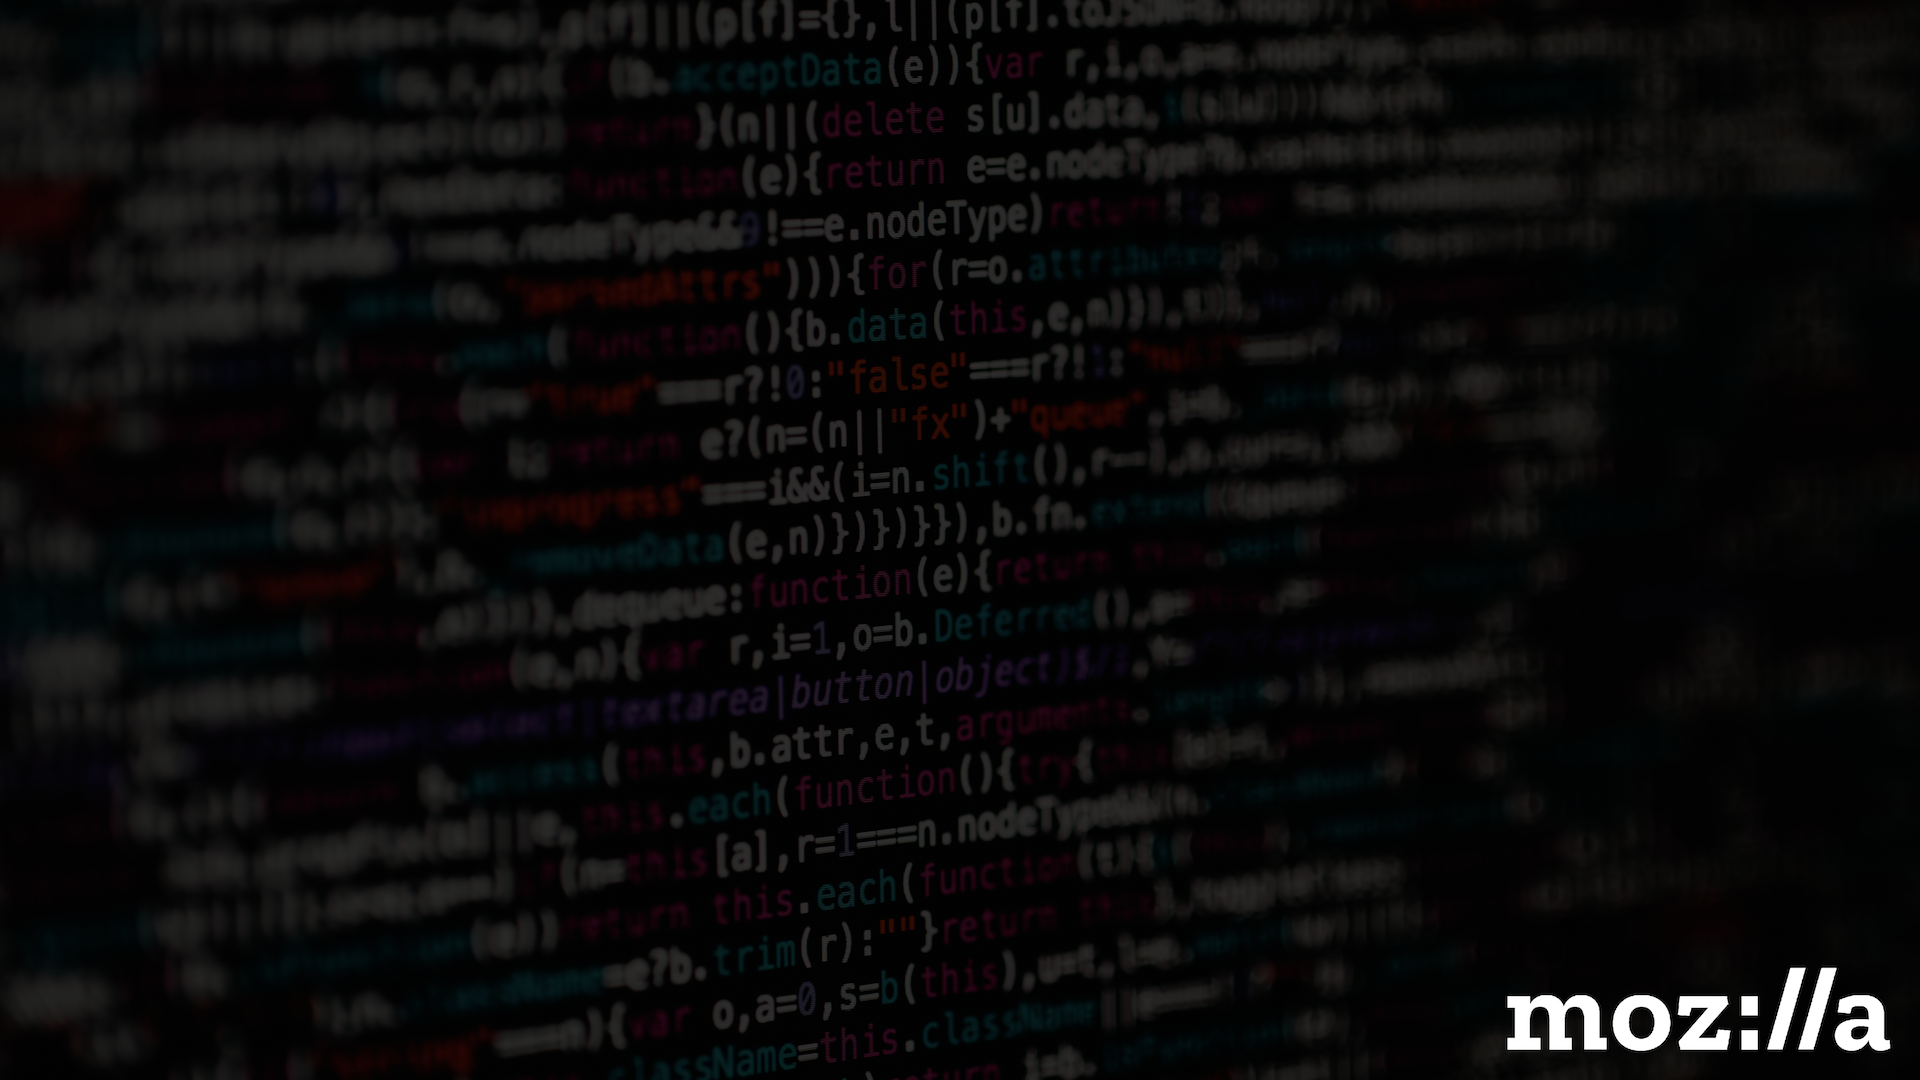
\includegraphics[width=\paperwidth]{bg_alt_small-rlogo.png}}%
\begin{frame}
\begin{overpic}[width=0.8\textwidth]{2015-web-large-2.png}
\put(-04.5,69.5){\textbf{THE INTERNET 2015}}
\put(-04.5,66){\tiny{Barrett Lyon / The Opte Project}}
%\blfootnote{Barrett Lyon / The Opte Project}
\end{overpic}
%This is our first full Internet map with color and other graphing logic. RFC1918 addresses have been hashed into a unique checksum so they do not incorrectly overlap with other routers or hosts. The checksums resolve to the same host each time to be sure that all routes connect correctly. Another bit of code also removed the routing loops that made a rather large mess out of previous maps. The colors were based on Class A allocation of IP space to different registrars in the world.
\end{frame}
}

\begin{frame}
\frametitle{The Centrality of Advertisers}
\large{Are trackers the new backbone of the Web?}
\begin{center}
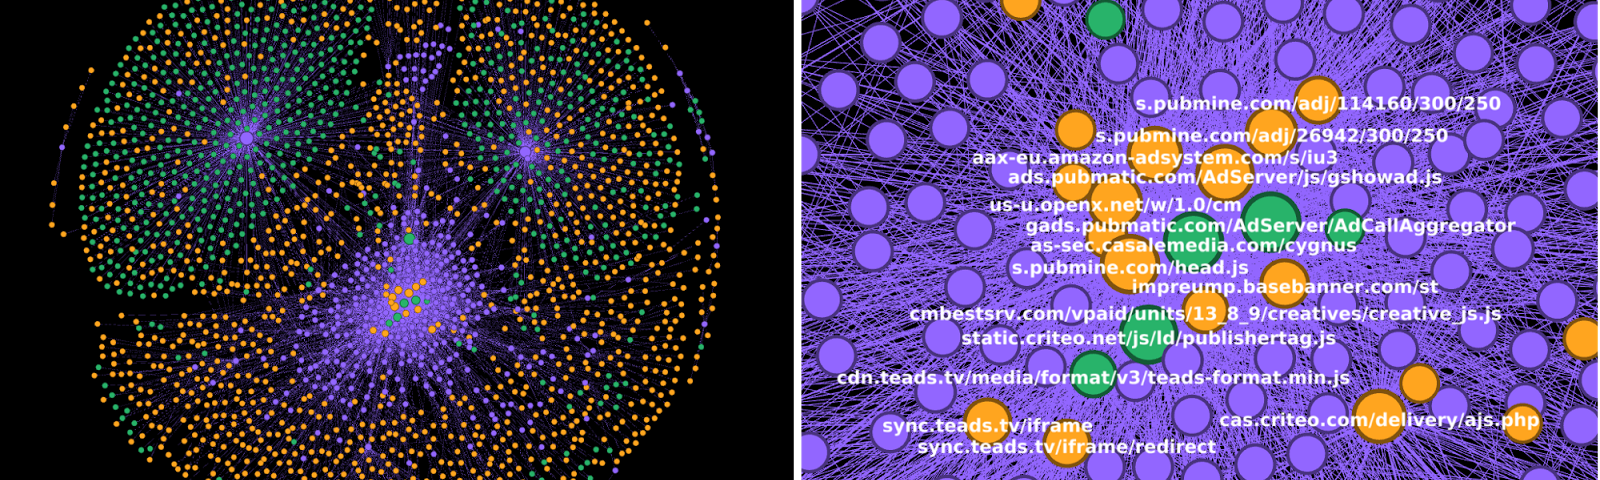
\includegraphics[width=0.85\paperwidth]{0thN-8lZ4H2_xjbkt.png}
\end{center}
% In 2017 we started working with students at the Information and Language Processing systems group at the University of Amsterdam, exploring the role of highly connected, hub nodes, among the most popular (or highly visited) websites on the Web at that time.

% As seen in the 2015 snapshot of the Web, we observed some hyper-connected nodes naturally 
%You don’t need cash to search Google or to use Facebook, but they’re not free. We pay for these services with our attention and with our data.

% In some examples, we observed substantially fewer hyperlinks between pages belonging to separate tracking communities than between pages tracked by a single % source of third-party resources. As the dynamic link generation is intended to keep attention in-ecosystem.
\end{frame}

\begin{frame}
\frametitle{How did we get to an ecosystem of silos?}
%We’ve already made some scary discoveries about the diversity of browsing behavior. A very early examination of a small group of Firefox users’, who voluntarily shared their browsing history, suggested that up to 
\begin{itemize}
\item{40\% of total Web browsing page views can be attributed to only 65 top level domains}
\item{Five (TLD+1) sites (Google, Facebook, Amazon, Yahoo, and Reddit) make up 22\% of all traffic}
% buisness model does not depend as much on 
\end{itemize}


\end{frame}

\begin{frame}
\frametitle{}
\epigraph{Social platforms were designed to facilitate; they became attention brokers, they are designed to help companies reach users as these sort of middlemen where they know a ton about you and thats the service they are providing to the advertisers.}{Renee DiResta on "The Internet's Original Sin\\ 27-Oct-2018 12:45}
% Ads alone aren't a problem, targeting is the problem. Social platforms are designed to collect attention and information in order to sell them to advertisers
% according to research cited in that talk 60% of people in the US get their news from Facebook,
\end{frame}

\begin{frame}
\frametitle{Outbound link types}
Retargetting
advertisment
realtime bidding
social linking

\end{frame}

\begin{frame}
\frametitle{}
\epigraph{I can't help but feel nauseous when I am loading independent.co.uk, Firefox literally grinds to a halt because of the extreme amount of tracking requests being logged in the browser console, and a popup shows up and says "We value your privacy"}{motin \\
28-Oct-2018 11:37}
%\blfootnote{https://github.com/motin}
\end{frame}


\begin{frame}
highest traffic pages on the internet are search engines, content aggregators, and commerce.
data stewardship
dynamic linking
\end{frame}

\begin{frame}
transparency, technolopgy, education

%Popularized by Berners-Lee's book Weaving the Web[32] and a Scientific American article by Berners-Lee, James Hendler, and Ora Lassila,[33] the term Semantic Web describes an evolution of the existing Web in which the network of hyperlinked human-readable web pages is extended by machine-readable metadata about documents and how they are related to each other, enabling automated agents to access the Web more intelligently and perform tasks on behalf of users. This has yet to happen. In 2006, Berners-Lee and colleagues stated that the idea "remains largely unrealized".[34]

% meaning that web crawls in the future will face the difficulty of increasingly complex algorithmic generation of outbound links.
% as the sophistication of 
\end{frame}

\begin{frame}
\frametitle{Challenges to crawl technology}
\begin{itemize}
\item{Limited View - the open web makes up less and less of the Web. Content Silos, }
\end{itemize}
% meaning that web crawls in the future will face the difficulty of increasingly complex algorithmic generation of outbound links.
% as the sophistication of 
\end{frame}


{
\usebackgroundtemplate{
\includegraphics[width=\paperwidth]{bg_last.png}}%
\begin{frame}

\end{frame}
}




\end{document}
